\documentclass[10pt]{article}
\usepackage[utf8]{inputenc}
\usepackage[english]{babel}
\usepackage{cite}
\usepackage[]{amsthm} %lets us use \begin{proof}
\usepackage[]{amssymb} %gives us the character \varnothing
\usepackage[ruled,vlined]{algorithm2e}
\usepackage{listings}
\usepackage[utf8]{inputenc}
\usepackage{hyperref} 
\usepackage{amsmath}
\usepackage{csvsimple}
\usepackage{graphicx}
% One inch margins
\PassOptionsToPackage{margin=0.25in}{geometry}
\title{Modern Optimization Final Exam}
\author{Guanhua Huang}
\date\today

\begin{document}
\maketitle %This command prints the title based on information entered above
All the source code is stored at \url{https://github.com/victorhuangkk/york_optimization_final}
There are five problems in total in this final exam. Please find them in the following. 

\begin{section}{Problem 9}
This is the problem \\
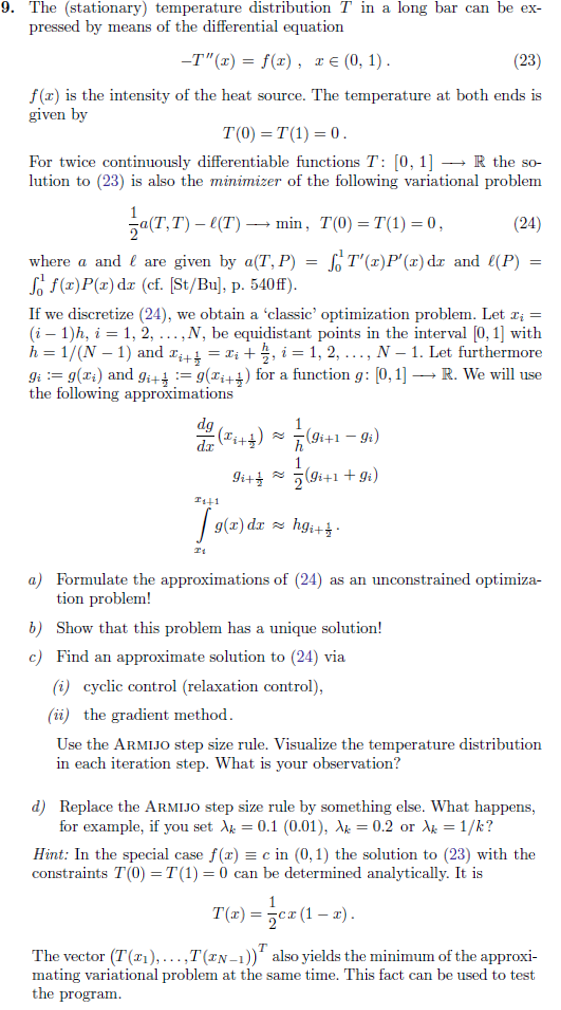
\includegraphics[width=5cm]{img/problem9.png}
\subsection{Part a}

Let's analyze the two parts separately, which are $a(T, T)$ and $l(T)$. Those two terms are generated by the variational method. 

\[\frac{1}{2}a(T, T) = \frac{1}{2} \int_{0}^{1}T^\prime(x)T^{\prime}(x) dx\]
\[l(T) = \int_{0}^{1} f(x)T(x)dx\]

Since we assume the second order differentiable, we can rewrite all the terms into a series of integral summations. For simplicity reasons, I would omit $\frac{1}{2}$ here, But in the quadratic optimization part, we can add it back. 
\[\frac{1}{2}a(T, T) = \frac{1}{2} \int_{0}^{1}T^\prime(x)T^{\prime}(x) dx\]
\[= \int_{0}^{x_1}(T^{\prime}(x))^2dx + \int_{x_1}^{x_2}(T^{\prime}(x))^2dx + ... \int_{x_{n-1}}^{x_n}(T^{\prime}(x))^2dx\]
\[\approxeq \sum_{i=1}^{N-1}h (T^{\prime}_{i+\frac{1}{2}})^2\]
\[\approxeq \sum_{i=1}^{N-1}h \frac{1}{h}(T_{i+1} - T_{i})\frac{1}{h}(T_{i+1} - T_{i})\]
\[= \sum_{i=1}^{N-1}\frac{1}{h}(T_{i+1} - T_{i})^2\]


And the approximation of $l(T)$ is done as below

\[\int_{0}^{1}f(x)T(x)dx = \int_{0}^{x_1}f(x)T(x)dx + \int_{x_1}^{x_2}f(x)T(x)dx + ... \int_{x_{n-1}}^{x_n}f(x)T(x)dx\]
\[= \sum_{i=1}^{N-1} \int_{x_i}^{x_{i+1}}f(x)T(x)dx\]
\[\approxeq \sum_{i=1}^{N-1} hf(x_{i+\frac{1}{2}})T(x_{i+\frac{1}{2}}), \;\;\; (\int_{x_i}^{x_{i+1}}g(x)dx \approxeq hg_{i+\frac{1}{2}} )\]

\[\approxeq h\sum_{i=1}^{N-1}\frac{1}{2} (f(x_i) + f(x_{i+1})) \frac{1}{2} (T(x_i) + T(x_{i+1}))\]

After combining these two terms together, we got the following approximation to the original objective function,
\[min(\frac{1}{h} \sum_{i=1}^{N-1}(T(x_{i+1}) - T(x_i))^2 - \frac{h}{4}\sum_{i=1}^{N-1} (f(x_i) + f(x_{i+1})) (T(x_i) + T(x_{i+1})))\]
\[s.t. \;\;\;\;\ T(0) = T(1) = 0\]

Then, in order to change the constraint optimization problem to an unconstrained version, Lagrange Multiple is used. 

\[min(\frac{1}{h} \sum_{i=1}^{N-1}(T(x_{i+1}) - T(x_i))^2 - \frac{h}{4}\sum_{i=1}^{N-1} (f(x_i) + f(x_{i+1})) (T(x_i) + T(x_{i+1})) + \lambda_0T(0) + \lambda_1T(1))\]

Because of the definition, $T(0) = T(x_1) = 0, T(1) = T(x_N) = 0$

To convert the polynomial to matrix format, let's rewrite the objective function by parts. 

\[\frac{1}{h} \sum_{i=1}^{N-1}(T(x_{i+1}) - T(x_i))^2 = \frac{1}{h} X^T A X\]
\[\frac{1}{h} (T_1^2 + 2T_2^2 + 2T_3^2 +... + 2(T_{N-1})^2 + (T_{N})^2 - 2T_1T_2 - 2T_2T_3 - .... - 2T_{N-1}T_{N})\]

One route to write the problem as an unconstrained problem is to do the following. Just to clarify here. $X = (T_1, T_2, T_3, ... T_{N-1}, T_N, \lambda_1, \lambda_N)^T$. This is the unknown vector we are trying to solve. However, $f(x_i)$ is a given value if $x_i$ is given. however, after 

So, in the end, the problem is formulated as the following: 
\[l(T, \lambda) = \frac{1}{2}\frac{1}{h} X^T A X + b^T X \to min\]

\subsection{Part b}
After transforming the original problem into a standard quadratic optimization problem, the uniqueness of solution can be proven by the positive definiteness of matrix A. To prove the positive definiteness, I would try to prove all the pivots of A (which is a symmetric square metrics) are positive. Then, the matrix is positive definite. 
\begin{proof}
	From linear algebra, we know that, in this scenario, A's quadratic summation can be written as
	\[x^T A x = \sum_{i=1}^{N-1}(x_{i+1} - x_{i})^2, \;\;\; \forall x_i \in \mathbf{x}\]
	if $\mathbf{x} \neq \mathbf{0}$, then $ \forall x, x^T A x >0$. For that reason, $A$ is positive definite. In quadratic programming, if $A$ is positive definite, there is a one and only one solution. Uniqueness is proven to be true. 
\end{proof}

\subsection{Part c}
As hinted by the instructor, $f(x) = c = 1$ to simplify the visualization. Coordinate descent and gradient descent are used to optimize the objective function respectively. For simplicity reason, I designate $N = 6$ such that $h = 0.2$. And there are six points at $x_1 = 0, x_2 = 0.2, x_3 = 0.4, x_4 = 0.6, x_5 = 0.8, x_6 = 1.0$. 

This is the exact temperature distribution over the bar, with the simple function $T(x) = \frac{1}{2}x(x-1)$\\
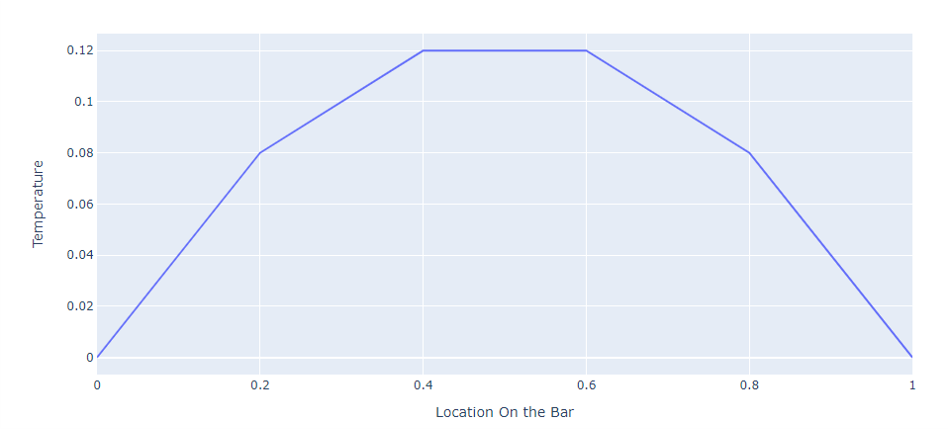
\includegraphics[width=10cm]{img/problem9_plt1.png}

\subsection{Part d}
The Armijo size rule has been replaced by the predefined step size and the results are summarized below. \\

\end{section}

\begin{section}{Problem 12}
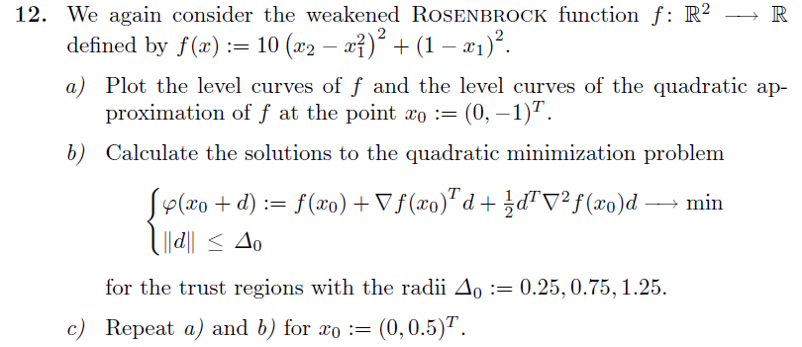
\includegraphics[width=10cm]{img/problem12.png}

\subsection{Part a}
The level plot of the function is shown below. The left hand side is the original function and the right hand side is the quadratic appropriation at $x_0 = (0, -1)^T$. \\

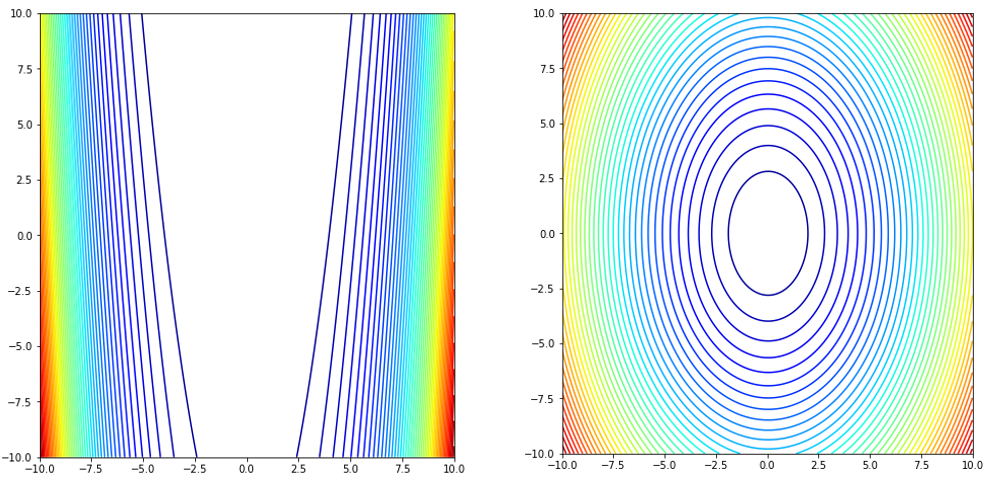
\includegraphics[width=12cm]{img/problem12_plt1.png}


\subsection{Part b}
The trust region method is implemented to solve this sub-problem
\lstinputlisting[language=python, basicstyle=\tiny]{src/trust_region.py}

Computational Results 


\begin{tabular}{lll}
	\hline
	$\Delta_0$ & $d_0$ & Steps Until Converge \\
	\hline\hline
	0.25 & (0.02, 0.249) & 2 \\
	0.75 & (0.048, 1.0)  & 1 \\
	1.25 & (0.048, 1.0)  & 1
\end{tabular}

\subsection{Part c}
The original function's level graph is the same but the quadratic approximation is different. \\
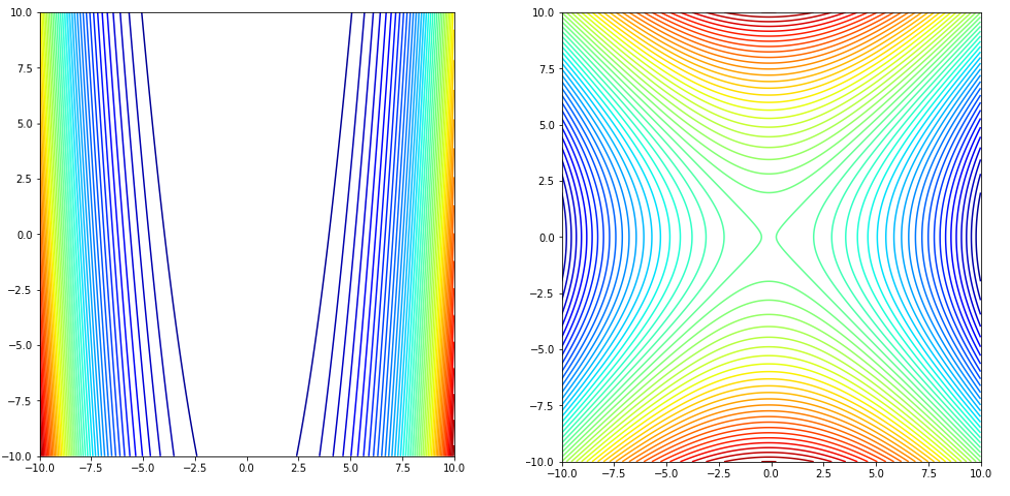
\includegraphics[width=12cm]{img/problem12_plt2.png}

The algorithm failed in this case since the hessian matrix is not positive definite such that Cholesky cannot be performed. 
\end{section}

\begin{section}{Problem 13}

   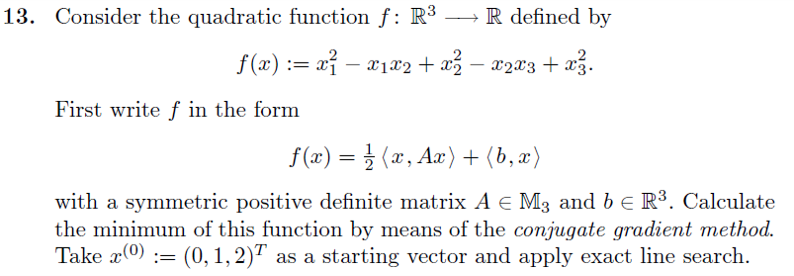
\includegraphics[width=10cm]{img/problem13.png}

    First, let's calculate A and b from the given formula:
    \[f(x) = \frac{1}{2}(x_1, x_2, x_3) \begin{pmatrix}
    a_1 & a_2 & a_3\\
    a_2 & a_4 & a_5 \\
    a_3 & a_5 & a_6 \end{pmatrix}
    \begin{pmatrix}
    x_1\\ 
    x_2 \\ x_3
    \end{pmatrix} + (b_1, b_2, b_3) \begin{pmatrix}
    x_1\\ x_2\\x_3  \end{pmatrix}\]
    
    Since there is no first order term in the final section, so, $b = (0, 0, 0)^T$
    \[\frac{1}{2}(a_1x_1+a_2x_2+a_3x_3, a_2x_1+a_4x_2+a_5x_3, a_3x_1+a_5x_2+a_6x_3)  \begin{pmatrix}
    x_1\\ 
    x_2 \\ x_3
    \end{pmatrix}\]
    
    \[=\frac{1}{2}x_1(a_1x_1+a_2x_2+a_3x_3) + 
    \frac{1}{2}x_2(a_2x_1+a_4x_2+a_5x_3) + 
    \frac{1}{2}x_3(a_3x_1+a_5x_2+a_6x_3)\]
    
    \[=\frac{1}{2}a_1x_1^2 + \frac{1}{2}a_4x_2^2 + \frac{1}{2}a_6x_3^2 + a_2x_1x_2 + a_3x_1x_3 + a_5x_2x_3\]
    \[=x_1^2 -x_1x_2 + x_2^2 -x_2x_3 + x_3^2\]
    
    For this reason, we know 
    $$A = \begin{pmatrix}
    	2 & -1 & 0\\
    	-1 & 2 & -1 \\
    	 0  & -1 & 2 \end{pmatrix}, \;\;\; b = \begin{pmatrix}
    	  0\\
    	  0 \\
    	  0 \end{pmatrix}$$
    
    The implementation is done in python and I pasted the code here for reference purposes. 
    \lstinputlisting[language=python, basicstyle=\small]{src/cg_algo.py}
    
    And the execution results is 

   	\begin{tabular}{llll}
   		\hline
   		Iteration & $x_0$ & $x_1$& $x_2$ \\
   		\hline\hline
   		0 & 0     & 1     & 2     \\
   		1 & 0.5   & 1     & 0.5   \\
   		2 & 0.556 & 0.444 & 0.333 \\
   		3 & 0     & 0     & 0    
   	\end{tabular}

\end{section}

\begin{section}{Problem 15}
	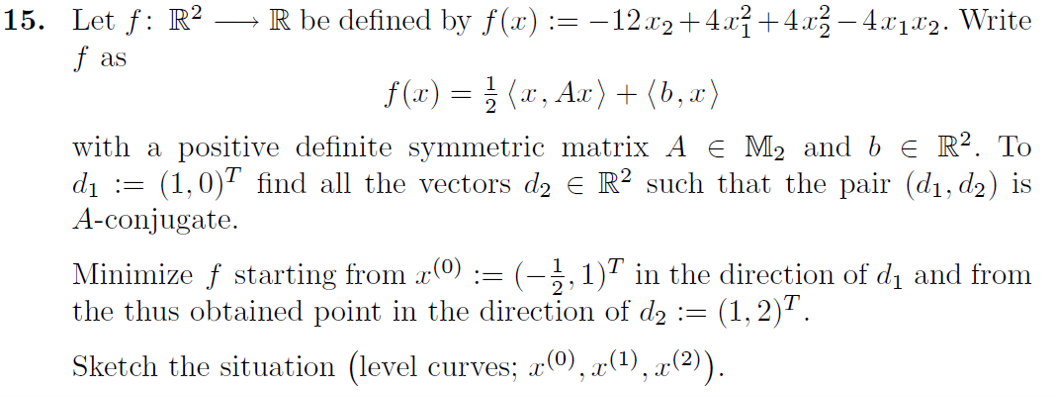
\includegraphics[width=12cm]{img/problem15.png}

	\subsection{Part 1}
	First, let's write the matrix format of the function,

	$$\frac{1}{2} (x_1, x_2) \begin{pmatrix}
	a_1 & a_2\\
	a_2 & a_3 \end{pmatrix}
	\begin{pmatrix}
	x_1\\ 
	x_2
	\end{pmatrix} + (b_1, b_2) \begin{pmatrix}
	x_1\\
	x_2
	\end{pmatrix}$$
	\[= \frac{1}{2}(a_1x_1 + a_2x_2, a_2x_1+a_3x_2) \begin{pmatrix}
	x_1\\
	x_2
	\end{pmatrix} + x_1b_1 + x_2b_2\]
	\[= \frac{1}{2}(a_1x_1 + a_2x_2)x_1 + \frac{1}{2}(a_2x_1 + a_3x_2)x_2 + x_1b_1 + x_2b_2\]
	\[= \frac{1}{2}a_1x_1^2 + a_2x_1x_2 + \frac{1}{2}a_3x_2^2 + b_1x_1 + b_2x_2\]
	\[=-12x_2 + 4x_1^2 + 4x_2^2-4x_1x_2\]	

	By comparing parameters, we got the following, 
	\[b_2 = -12, b_1 = 0, a_2 = -4, a_1 =a_3 = 8\]
	\[A = \begin{pmatrix}
	8 & -4\\
	-4 & 8
	\end{pmatrix}, b = \begin{pmatrix}
	0\\
	-12
	\end{pmatrix}\]
	
	Based on A-conjugate definition (on page 120), $\langle d_1, Ad_2 \rangle = 0, \;\; d_1 = (1,0)^T$, then, let's write out the problem as the following: 
	
	$$(1,0) \begin{pmatrix}
	8 & -4\\
    -4 & 8 \end{pmatrix} \begin{pmatrix}
	\delta_1\\
     \delta_2 \end{pmatrix} = (8, -4) \begin{pmatrix}
     \delta_1\\
     \delta_2 \end{pmatrix} = 8\delta_1 - 4\delta_2 = 0$$
    So, as long as $2\delta_1 = \delta_2$, the condition $\langle d_1, Ad_2 \rangle = 0$ is satisfied
    $$d_2 = \begin{pmatrix}
    \gamma\\
    2\gamma \end{pmatrix}, \;\; \forall \gamma \in \mathbb{R}$$	
	\subsection{Part 2}
	
	Let's calculate the gradient of the function,
	\[f(x) = -12x_2 + 4x_1^2 + 4x_2^2-4x_1x_2, \;\; \nabla f(x) = \begin{pmatrix}
	8x_1 - 4x_2\\
	-12 + 8x_2 - 4x_1 \end{pmatrix} = g(x)\]
	
	Then, we can evaluate $g_0 = \begin{pmatrix}
	-\frac{1}{2} \times 8 - 4 \times 1\\
	-12 + 8 + 2
	\end{pmatrix} = \begin{pmatrix}
	-8\\
	-2
	\end{pmatrix}$ by given $x_0 = \begin{pmatrix}
	-\frac{1}{2}\\
	1
	\end{pmatrix}$
	
	In this problem, $d_1$ is given so we don't have to calculate it by $g_0$. So, the next stuff we need is the $\lambda_0 = -\frac{ \langle g_0, d_0 \rangle}{\langle Ad_0, d_0\rangle}$. I would calculate the numerator and enumerator separately.
	
	\[-\langle g_0, d_0 \rangle = -(-8, -2) \begin{pmatrix}
	1\\
	0
	\end{pmatrix} = 8\] 
	\[\langle Ad_0, d_0 \rangle  = (1,0) \begin{pmatrix}
	8 & -4\\
	-4 & 8
	\end{pmatrix} \begin{pmatrix}
	1\\
	0
	\end{pmatrix} = (8, -4) \begin{pmatrix}
	1\\
	0
	\end{pmatrix} = 8\]
	
	For this reason, $\lambda_0 = \frac{8}{8}=1$, and $x^{(1)}$ is, 
	\[x^{(1)} = \begin{pmatrix}
	-1/2\\
	1
	\end{pmatrix} + 1 \begin{pmatrix}
	1\\
	0
	\end{pmatrix} = \begin{pmatrix}
	\frac{1}{2}\\
	1
	\end{pmatrix} \]
	
	In the next iteration, we calculate $x^{(2)}$. To accomplish that, we calculate $g_1 = \begin{pmatrix}
	\frac{1}{2} \times 8 - 4 \times 1\\
	-12 + 8 - 4 \times \frac{1}{2}
	\end{pmatrix} = \begin{pmatrix}
	0\\
	-6
	\end{pmatrix}$
	
	and by given in the problem, we know $d_1 = \begin{pmatrix}
	1\\
	2
	\end{pmatrix}$, I follow the same routine to calculate the $\lambda_1$
	\[-\langle g_1, d_1 \rangle = -(0, -6) \begin{pmatrix}
	1\\
	2
	\end{pmatrix} = 12\] 
	
	\[\langle Ad_0, d_0 \rangle  = (1,2) \begin{pmatrix}
	8 & -4\\
	-4 & 8
	\end{pmatrix} \begin{pmatrix}
	1\\
	2
	\end{pmatrix} = (0, 12) \begin{pmatrix}
	1\\
	2
	\end{pmatrix} = 24\]
	
	For this reason, $\lambda_1 = \frac{1}{2}$ and we can evaluate $x^{(2)}$ as
	\[x^{(2)} = \begin{pmatrix}
	1/2\\
	1
	\end{pmatrix} + \frac{1}{2} \begin{pmatrix}
	1\\
	2
	\end{pmatrix} = \begin{pmatrix}
	1\\
	2
	\end{pmatrix} \]
	 
	\subsection{Part 3}
	The visualization has been done in python via matplotlib. Please refer to the source code to see details. Here is the plot. 

		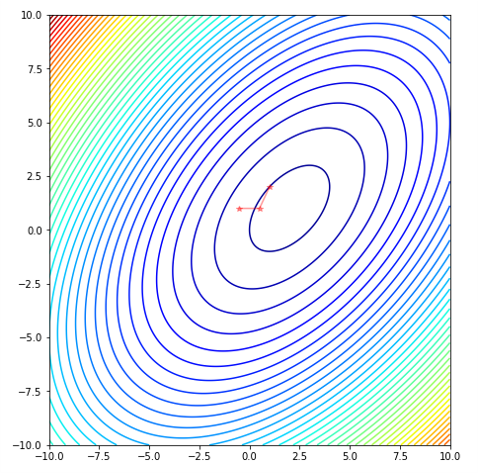
\includegraphics[width=8cm]{img/problem15_plt1.png}


\end{section}

\begin{section}{Problem 18}
	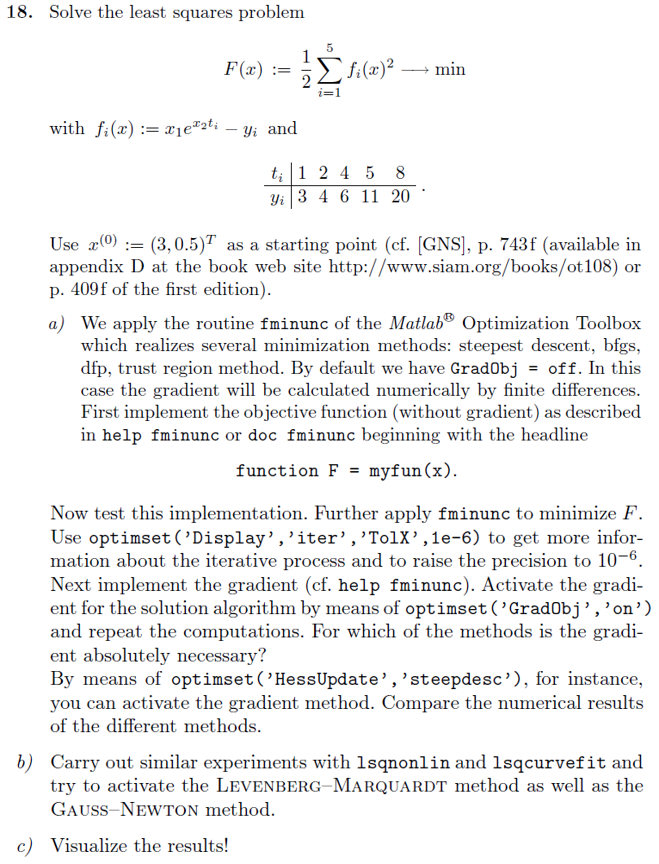
\includegraphics[width=10cm]{img/problem18.png}
	\subsection{Part a}
	First, followed by the hints posted on the website, I tested the four methods, which are ,Newton-cg, trust-ncg, trust-krylov, and trust-exact in scipy with tolerance $10^{-6}$. All results are summarized below. To make sure all methods works fine, the original function, Jacobian and Hessian are all provided to the program. In terms of details, please refer to the source code. 

    	\begin{tabular}{lllll}
    		\hline
    		Method &Iterations & $x_1$ & $x_2$& Function Value \\
    		\hline\hline
			newton-cg  & 14  & 2.541  & 0.260& 2.247    \\
			trust-ncg       & 15   & 2.541  & 0.260 & 2.247    \\
			trust-krylov    & 21   & 2.541  & 0.260 & 2.247 \\
			trust-exact     & 14  & 2.541  & 0.260 & 2.247
    	 \end{tabular}
     
    So, all the methods generated the same results.  
	\subsection{Part b}
	The least square result is summarized here, three methods were used as requested by the instructor. The objective function is different from part a, but just the residual of the least square function. After fitting, here are the results. 
	
	\begin{tabular}{lllll}
		\hline
		Method &Iterations & $x_1$ & $x_2$& Function Value \\
		\hline\hline
		trf  & 8  & 2.541  &  0.260 & $5.159\times 10^{-5}$  \\
		dogbox & 8   & 2.541  &   0.260 & $5.167\times 10^{-5}$  \\
		lm    & 22   & 2.541  &  0.260 & $5.179\times 10^{-5}$
	\end{tabular}

	
	\subsection{Part c}
	The ultimate goal is to estimate parameters and fit the five data points. The graph below is the visualization in part a and b. Since all the parameters are the same, I used only one plot here for simplification. 
	
	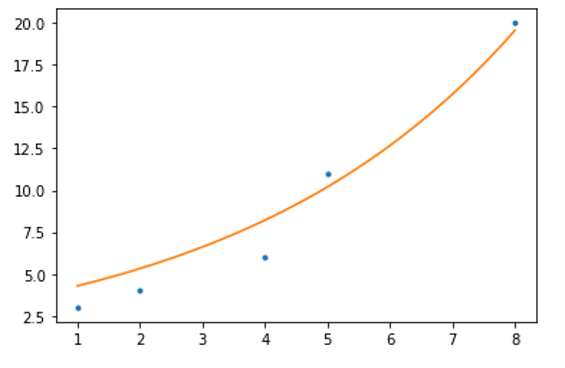
\includegraphics[width=10cm]{img/problem18_plt1.png}
	
\end{section}




\end{document}